\documentclass[hidelinks,a4paper,12pt, nofootinbib]{article}
\usepackage[width=15.5cm, left=3cm, top=2.5cm, right=2cm, left=2cm, height= 24.5cm]{geometry}
\usepackage[spanish, es-tabla]{babel} %es-tabla es para que ponga Tabla en vez de Cuadro en el caption
\usepackage[utf8]{inputenc}
\usepackage[T1]{fontenc}
\usepackage{xspace}
\usepackage{xargs}
\usepackage{fancyhdr}
\usepackage{lastpage}
\usepackage{caratula}
\usepackage[bottom]{footmisc}
\usepackage{amsmath}
\usepackage{amssymb}
\usepackage{algorithm}
\usepackage[noend]{algpseudocode}
\usepackage{array}
\usepackage{xcolor,colortbl}
\usepackage{amsthm}
\usepackage{listings}
\usepackage{graphicx}
\usepackage{sidecap}
\usepackage{wrapfig}
\usepackage{caption}

%%fancyhdr
\pagestyle{fancy}
\thispagestyle{fancy}
\addtolength{\headheight}{1pt}
\lhead{Sistemas Operativos: TP1}
\rhead{$1º$ cuatrimestre de 2016}
\cfoot{\thepage\ / \pageref{LastPage}}
\renewcommand{\footrulewidth}{0.4pt}
\renewcommand{\labelitemi}{$\bullet$}

% Datos de caratula
\materia{Sistemas Operativos}
\titulo{Trabajo Práctico 1}
\subtitulo{Scheduling}
\grupo{}

\integrante{Costa, Manuel José Joaquin}{035/14}{manucos94@gmail.com}
\integrante{Coy, Camila}{}{}
\integrante{Ginsberg, Mario Ezequiel}{145/14}{ezequielginsberg@gmail.com}

\fecha{2 de Mayo de 2016}

\begin{document}
\maketitle
\tableofcontents
\newpage

\clearpage

\section{Ejercicio 1}
\begin{figure}[H]
  \centering
  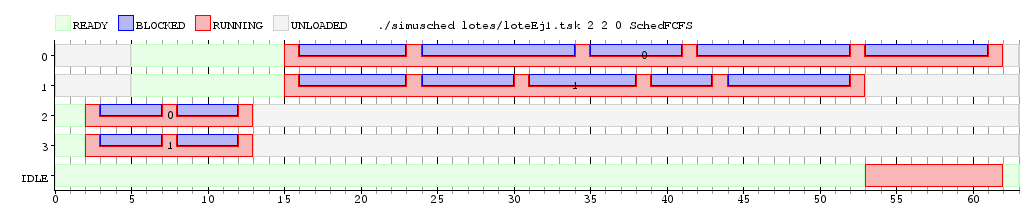
\includegraphics[width=\textwidth]{img/imgEj1-1.png}
  \caption{}
  \label{fig:ej1}
\end{figure}
\newpage

\section{Ejercicio 2}
\begin{figure}[H]
  \centering
  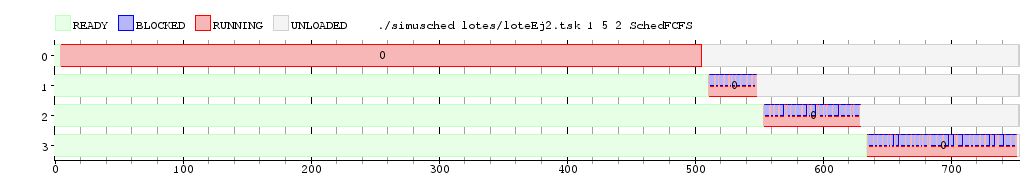
\includegraphics[width=1\textwidth]{img/imgEj2-1}
  \caption{}
  \label{fig:ej2-1}
\end{figure}

\begin{figure}[H]
  \centering
  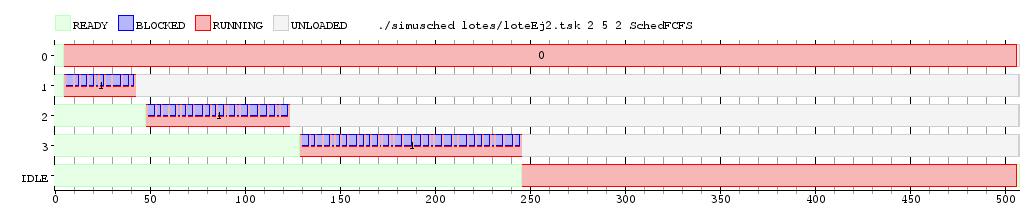
\includegraphics[width=1\textwidth]{img/imgEj2-2}
  \caption{}
  \label{fig:ej2-2}
\end{figure}

\begin{figure}[H]
  \centering
  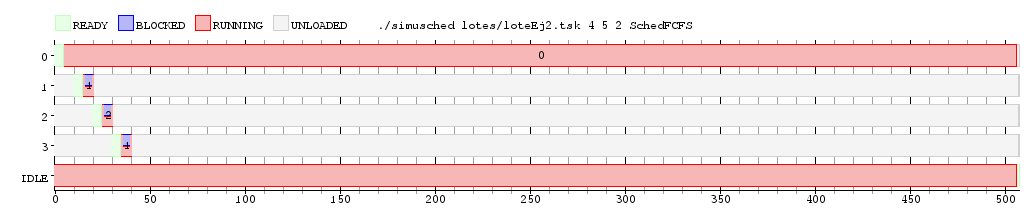
\includegraphics[width=1\textwidth]{img/imgEj2-3}
  \caption{}
  \label{fig:ej2-3}
\end{figure}
\newpage

\section{Ejercicio 3}
\begin{figure}[H]
  \centering
  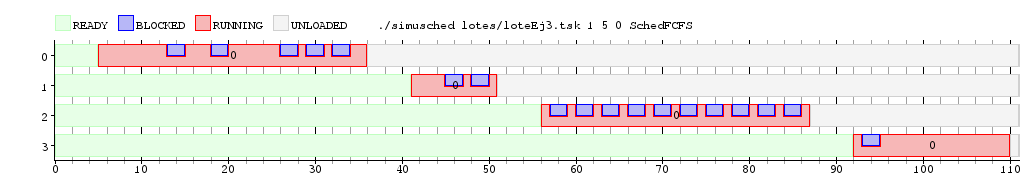
\includegraphics[width=1\textwidth]{img/imgEj3}
  \caption{}
  \label{fig:ej3}
\end{figure}
\newpage

\section{Ejercicio 4}
A continuación detallamos los atributos privados de la clase \texttt{SchedRR}:
\begin{itemize}
	\item \texttt{cant\_cores}: almacena la cantidad de procesadores que tiene el sistema.
	\item \texttt{cola\_procesos}: la cola \emph{FIFO} en la cual se almacenan todos los procesos que están cargados, listos para ejecutar (o sea, en estado \emph{ready}). Dicha cola es global para todos los procesadores.
	\item \texttt{quantum\_original\_cpu}: es un vector de longitud \texttt{cant\_cores}, tal que \texttt{quantum\_original\_cpu[i]} indica la duración de un \emph{quantum} del procesador \texttt{i}.
	\item \texttt{quantum\_restante\_cpu}: otro vector de longitud \texttt{cant\_cores}, tal que \texttt{quantum\_restante\_cpu[i]} indica cuántos ciclos le quedan al proceso corriendo en el procesador \texttt{i} antes de agotar su \emph{quantum}. En el caso en que se esté corriendo la tarea \emph{idle} este valor no representa nada (pues tal tarea debe correr indefinidamente hasta que aparezca una nueva tarea para ser ejecutada).
\end{itemize}

Además, la clase cuenta con una función auxiliar, \texttt{int next(int cpu)}, que se encarga de devolver el \emph{pid} del siguiente proceso a ejecutar, removiéndolo de la cola de procesos y reiniciando el \emph{quantum} disponible para el proceso que llega. Notar que en caso de que no hayan procesos en \emph{ready} los últimos dos pasos no se ejecutan y simplemente se devuelve el \emph{pid} de la tarea \emph{idle}.

La clase posee los siguientes métodos públicos:
\begin{itemize}
	\item \texttt{void load(int pid)}: se encarga de cargar el proceso identificado por \texttt{pid}. Notar que esto simplemente consiste en agregarlo a la cola. Luego, eventualmente se ejecutará en un tick de reloj.
	\item \texttt{void unblock(int pid)}: vuelve a cargar una tarea que dejó de estar bloqueada, lo que consiste simplemente en llamar a la función \texttt{load}.
	\item \texttt{int tick(int cpu, const enum Motivo m)}: esta función se divide en tres casos según el motivo con el que se la haya llamado. Tanto en el caso en que la tarea que corría en \texttt{cpu} se haya bloqueado como en el que terminó hacemos lo mismo: sencillamente ponemos a correr a la siguiente tarea disponible (o a \emph{idle} en caso de no haber ninguna), dejando a la tarea actual fuera del ciclo de ejecución (temporalmente en un caso, permanentemente en el otro). Si no sucedieron ninguna de las dos cosas entonces tenemos nuevamente tres posibles escenarios:
	\begin{enumerate}
		\item La tarea actual es \emph{idle}, en cuyo caso solo queda llamar a \texttt{next} y devolver su resultado.
		\item La tarea actual no es \emph{idle} pero agotó su \emph{quantum}, por lo que la volvemos a encolar (pues aún no ha terminado) y llamamos a \texttt{next}. Si no había otra tarea se seguirá ejecutando la misma durante otro \emph{quantum}.
		\item La tarea actual ni es \emph{idle} ni terminó su \emph{quantum}, así que debe seguir ejecutando pero reducimos en 1 la cantidad de ciclos restantes.
	\end{enumerate}
\end{itemize}
\newpage

\section{Ejercicio 5}
\begin{figure}[H]
  \centering
  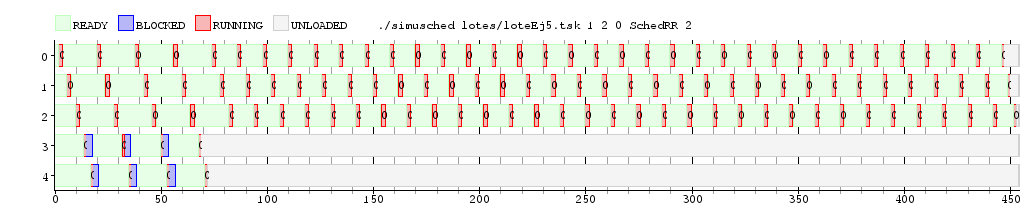
\includegraphics[width=1\textwidth]{img/imgEj5-1}
  \caption{}
  \label{fig:ej5-1}
\end{figure}

\begin{figure}[H]
  \centering
  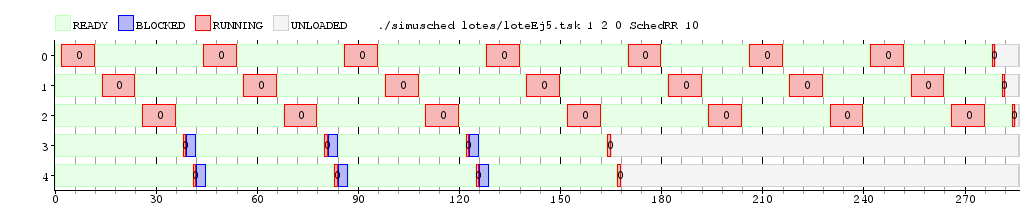
\includegraphics[width=1\textwidth]{img/imgEj5-2}
  \caption{}
  \label{fig:ej5-2}
\end{figure}

\begin{figure}[H]
  \centering
  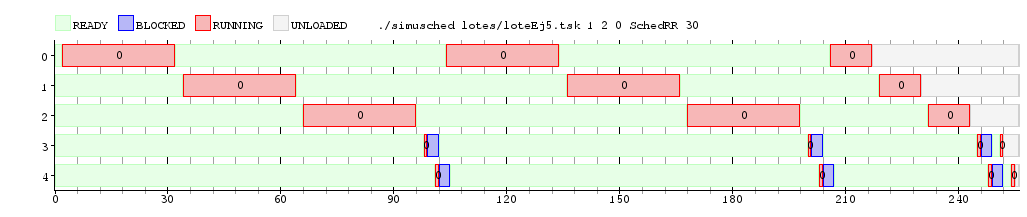
\includegraphics[width=1\textwidth]{img/imgEj5-3}
  \caption{}
  \label{fig:ej5-3}
\end{figure}

\begin{table}[H]
  \center
  \begin{center}
  \begin{tabular}{c|c|c|c|}
    \cline{2-4}
    & \multicolumn{3}{|c|}{\cellcolor{LightCyan}Latencia} \\
    \hline
    \rowcolor{LightCyan}
    \multicolumn{1}{|c|}{Quantum} & 2 & 10 & 30 \\
    \hline
    \multicolumn{1}{|c|}{\cellcolor{LightCyan}Tarea 0} & 2 & 2 & 2 \\
    \multicolumn{1}{|c|}{\cellcolor{LightCyan}Tarea 1} & 6 & 14 & 34 \\
    \multicolumn{1}{|c|}{\cellcolor{LightCyan}Tarea 2} & 10 & 26 & 66 \\
    \multicolumn{1}{|c|}{\cellcolor{LightCyan}Tarea 3} & 15 & 39 & 99 \\
    \multicolumn{1}{|c|}{\cellcolor{LightCyan}Tarea 4} & 18 & 42 & 101 \\
    \hline
    \multicolumn{1}{|c|}{\cellcolor{LightCyan}Promedio} & 10.2 & 24.6 & 60.4 \\
    \hline
  \end{tabular}
  \end{center}
  \caption{\footnotesize Latencia de cada tarea y latencia promedio según la duración del \emph{quantum} utilizado.}
  \label{tab:ej5-1}
\end{table}

\begin{table}[H]
  \center
  \begin{center}
  \begin{tabular}{c|c|c|c|}
    \cline{2-4}
    & \multicolumn{3}{|c|}{\cellcolor{LightCyan}\emph{Waiting time}} \\
    \hline
    \rowcolor{LightCyan}
    \multicolumn{1}{|c|}{Quantum} & 2 & 10 & 30 \\
    \hline
    \multicolumn{1}{|c|}{\cellcolor{LightCyan}Tarea 0} & ? & ? & ? \\
    \multicolumn{1}{|c|}{\cellcolor{LightCyan}Tarea 1} & ? & ? & ? \\
    \multicolumn{1}{|c|}{\cellcolor{LightCyan}Tarea 2} & ? & ? & ? \\
    \multicolumn{1}{|c|}{\cellcolor{LightCyan}Tarea 3} & ? & ? & ? \\
    \multicolumn{1}{|c|}{\cellcolor{LightCyan}Tarea 4} & ? & ? & ? \\
    \hline
    \multicolumn{1}{|c|}{\cellcolor{LightCyan}Promedio} & ? & ? & ? \\
    \hline
  \end{tabular}
  \end{center}
  \caption{\footnotesize Tiempo total de ejecución de cada tarea (\emph{turn-around}) y promedio según la duración del \emph{quantum} utilizado.}
  \label{tab:ej5-2}
\end{table}

\begin{table}[H]
  \center
  \begin{center}
  \begin{tabular}{c|c|c|c|}
    \cline{2-4}
    & \multicolumn{3}{|c|}{\cellcolor{LightCyan}\emph{Turn-around}} \\
    \hline
    \rowcolor{LightCyan}
    \multicolumn{1}{|c|}{Quantum} & 2 & 10 & 30 \\
    \hline
    \multicolumn{1}{|c|}{\cellcolor{LightCyan}Tarea 0} & 447 & 279 & 217 \\
    \multicolumn{1}{|c|}{\cellcolor{LightCyan}Tarea 1} & 450 & 282 & 230 \\
    \multicolumn{1}{|c|}{\cellcolor{LightCyan}Tarea 2} & 453 & 285 & 243 \\
    \multicolumn{1}{|c|}{\cellcolor{LightCyan}Tarea 3} & 69 & 165 & 252 \\
    \multicolumn{1}{|c|}{\cellcolor{LightCyan}Tarea 4} & 72 & 168 & 255 \\
    \hline
    \multicolumn{1}{|c|}{\cellcolor{LightCyan}Promedio} & 298.2 & 235.8 & 239.4 \\
    \hline
  \end{tabular}
  \end{center}
  \caption{\footnotesize Tiempo total de ejecución de cada tarea (\emph{turn-around}) y promedio según la duración del \emph{quantum} utilizado.}
  \label{tab:ej5-3}
\end{table}

%EN el primer caso gasto lo mismo en CS que en CPU
\newpage

\section{Ejercicio 6}
En la figura \ref{fig:ej6-1} se ilustra el mismo lote que en el punto anterior, pero ahora usando el \emph{scheduler FCFS}.

\begin{figure}[H]
  \centering
  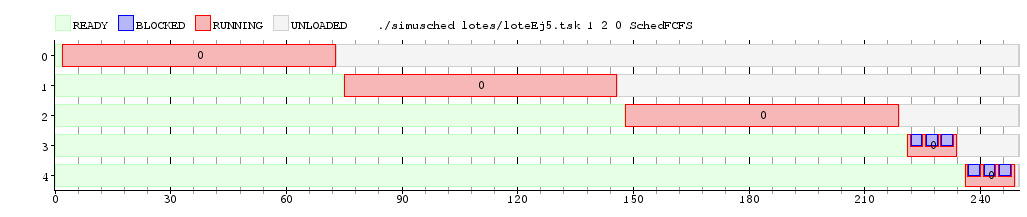
\includegraphics[width=1\textwidth]{img/imgEj6-1}
  \caption{}
  \label{fig:ej6-1}
\end{figure}

Una de las diferencias entre ambos schedulers es que el tiempo total que se requiere para ejecutar todo el lote es siempre menor con una estrategia FCFS. Esto se debe a que este algoritmo de \emph{scheduling} realiza la mínima cantidad de cambios de contexto posibles (uno por cada proceso involucrado).

Al mismo tiempo empeora mucho la latencia de las tareas respecto a \emph{Round Robin}. Además, con FCFS, esta métrica depende fuertemente del orden de llegada de los procesos, pues hay una gran diferencia entre que lleguen las tareas en orden creciente de tiempo de ejecución (mejor caso), y lo opuesto (peor caso, figura \ref{fig:ej6-1}). En ese sentido, \emph{Round Robin} es más robusto pues la latencia de los procesos depende mucho menos del orden de llegada y más de la duración del \emph{quantum} (lo que resulta mucho más manejable). 

En la figura \ref{fig:ej6-2} se grafica el mismo lote de tareas para FCFS pero cambiando el orden de llegada por el de mejor caso. Una buena forma de notar la diferencia en las latencias respecto del gráfico \ref{fig:ej6-1} es comparar la latencia del proceso con máxima latencia de cada gráfico, es decir el último en ejecutar en cada caso.

\begin{figure}[H]
  \centering
  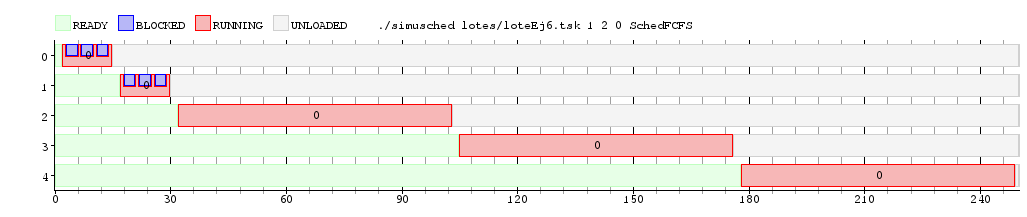
\includegraphics[width=1\textwidth]{img/imgEj6-2}
  \caption{}
  \label{fig:ej6-2}
\end{figure}


\newpage

\section{Ejercicio 7}
Después de varias pruebas descubrimos que el comportamiento de \texttt{SchedMistery} tiene el compartamiento de un \emph{multilevel feedback-queue}. Los parametros pasados son los quantums de las colas en orden de mayor a menos prioridad y tiene por defecto una cola de quantum 1 que es la de mayor prioridad.
\newline Detallamos los atributos privados y las funciones publicas de la clase \texttt{SchedNoMistery} donde replicamos el comportamiento de \texttt{SchedMistery}
Atributos privados:
\begin{itemize}
	\item \texttt{vq}: Es un vector que tiene las colas de prioridad en orden, la de mayor prioridad en el 0 y la de menor al final.
	\item \texttt{def\_quantum}: Tiene el quantum de cada una de las colas en vq. La cola en el subíndice i de vq tiene su respectivo quantum en el subíndice i de def\_quantum. 
	\item \texttt{unblock\_to}: Un vector hay un subíndice para cada proceso que tenga el procesador. Cuando un proceso se bloquea guarda en el subíndice pid la prioridad que le toca al desbloquearse. Esto funciona ya que los id de procesos empiezan en 0 y aumentan de a uno a medida que llegan.
	\item \texttt{quantum}: El quantum que le queda a el proceso que esta corriendo.
	\item \texttt{n}: La  cantidad de colas que tiene el scheduler.
	\item \texttt{cur\_pri}: La prioridad de la proceso que se esta corriendo
\end{itemize}

La clase tiene una función privada, \texttt{int next()}, que se encarga de devolver el \emph{pid} del siguiente proceso a ejecutar, buscado, desde la cola de mayor prioridad hasta la de menor, la primera cola vacia donde remueve el primer procesos, reinicia el \emph{quantum} y actualiza \emph{cur\_pri}. En caso de que todas las colas esten vacias devuelve el \emph{pid} de la tarea \emph{idle}.

Además posee los siguientes métodos públicos:
\begin{itemize}
	\item \texttt{SchedNoMistery(vector<int> argn)}: El constructor lee los quantum de las colas pasados como parámetros y los coloca en orden en def\_quantum y genera una cola vacia  para cada cola en vq, para así poder acceder más tarde. Además inicializa cur\_pri con 0, quantum como 1 y n como la cantidad de colas.
	\item \texttt{void load(int pid)}: Carga el proceso identificado por \texttt{pid} en la cola de mayor prioridad. 
	\item \texttt{void unblock(int pid)}: Agrega el proceso con id \texttt{pid} en la cola de prioridad indicada por el contenido del subíndice pid de \texttt{unblock\_to}.
	\item \texttt{int tick(int cpu, const enum Motivo m)}: Tiene tres casos según el motivo con el que se la haya llamado:
	\begin{enumerate}
		\item \texttt{Caso EXIT}: Simplemente llamamos a \texttt{next()} para que corra el siguiente proceso.
		\item \texttt{Caso BLOCK}: Guardo en \texttt{unblock\_to} en la posición del id del proceso que se corre, la prioridad actual menos uno. Después se llama a \texttt{next()} para que pueda correr el siguiete proceso.
		\item \texttt{TICK}: Pueden pasar varias cosas:
		\begin{enumerate}
			\item La tarea actual es \emph{idle}, en cuyo caso solo queda llamar a \texttt{next} y devolver su resultado.
			\item La tarea actual no es \emph{idle} pero se acabó su \emph{quantum}, por lo que hay que encolarla en la siguiente cola con menor prioridad y llamamos a \texttt{next}.
			\item La tarea actual ni es \emph{idle} ni terminó su \emph{quantum}, así que debe seguir ejecutando pero reducimos en 1 la cantidad de ciclos restantes.
		\end{enumerate}
	\end{enumerate}
\end{itemize}

Los diagramas \ref{fig:ej7-1} \ref{fig:ej7-2} \ref{fig:ej7-3} son los que más nos ayudaron para darnos cuenta como funcinaba \texttt{SchedMistery}.

\begin{figure}[H]
  \centering
  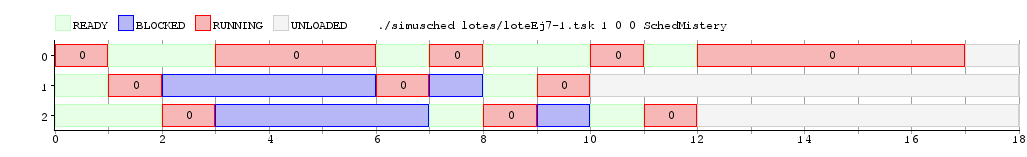
\includegraphics[width=1\textwidth]{img/imgEj7-1}
  \caption{}
  \label{fig:ej7-1}
\end{figure}

Para este diagrama no pasamos ningún parametro a \texttt{SchedMistery} lo que nos mostro que siempre tiene una cola de 1 de quantum. 

\begin{figure}[H]
  \centering
  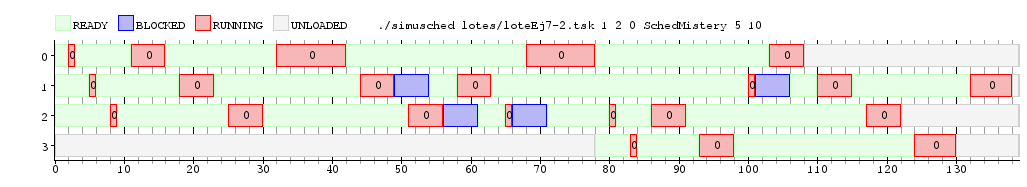
\includegraphics[width=1\textwidth]{img/imgEj7-2}
  \caption{}
  \label{fig:ej7-2}
\end{figure}

En este diagrama los quantums de las colas son 1, 5 y 10. Podemos observar que los tres procesos empiezan ejecutando quantum 1, después pasan a la segunda cola y ejecutan por 5 ciclos pasando a la tercera cola donde el proceso 0 gasta todo su quantum pero los procesos 1 y 2 se bloquean. Estos procesos pasan a la segunda cola, aumentando su prioridad, por eso el proceso 1 corre 5 ciclos, en cambio el proceso 2  se vuelve a bloquear y pasa a la primera cola. Como el proceso 1 entro último a la cola de menor prioridad y el proceso 2 esta bloqueado ejecuta el proceso 0. En el tiempo 78 entra el proceso 3 y se ubica al final de la primera cola, por esto se ejecuta el 2 (que había subido dos grados su prioridad) y luego el 3. Con esto pudimos ver que al gastar todo su quantum pasa a la siguiente cola con menor prioridad y al bloquearse  pasa a la siguiente cola con mayor prioridad.

\begin{figure}[H]
  \centering
  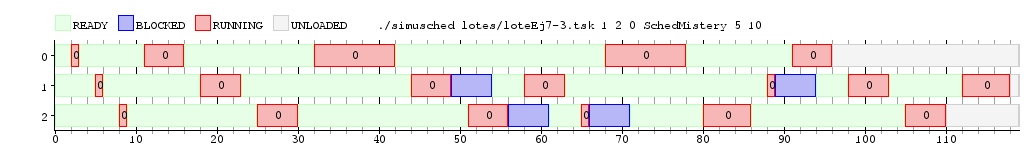
\includegraphics[width=1\textwidth]{img/imgEj7-3}
  \caption{}
  \label{fig:ej7-3}
\end{figure}

El lote usado para este diagrama es muy similar al anterior, la única diferencia es que no se agrega el proceso 3 en el tiempo 78. Esto genera que el proceso 2 cuando empieza a ejecutarse en el tiempo 80 ejecuta su quantum de 1 y como después de esto sigue siendo el más prioritario vuelve a ejecutar con el quantum de la segunda cola de prioridad (5), por eso ejecuta un total de 6 ciclos. Este gráfico nos mostro que para buscar al próximo proceso para ejecutarse siempre empezaba buscando en la cola de mayor prioridad hasta encontrar una cola que no estuviera vacia. Por lo que no ejecuta los de menor prioridad hasta acabar con los de mayor prioridad.
\newpage

\section{Ejercicio 8}
\subsection{Introducci\'on} En este ejercicio se nos propone implementar un scheduler $Round$-$Robin$ que no permita migraci\'on de procesos (al contrario del $Round$-$Robin$ del ejercicio 4), y cumpliendo una serie de otras caracter\'isticas, como que la asignaci\'on de CPU se realiza al momento que se carga el proceso, y que se elige a la CPU que tiene menor cantidad de procesos activos totales (RUNNING + BLOCKED + READY).

\subsection{Estructura Interna} Para resolver el problema, elegimos la siguiente estructura interna:
\begin{itemize}
	\item \texttt{cant\_cores}: Un n\'umero entero que indica la cantidad de n\'ucleos del procesador.
	\item \texttt{cola\_procesos\_cpu}: Un vector de colas de enteros que guarda, para cada cpu (numeradas del 0 a cant\_cores-1), su correspondiente cola de procesos en el estado de ready.
	\item \texttt{quantum\_original\_cpu}: Un vector de enteros que guarda, para cada cpu, su correspondiente quantum. Notar que esta variable no se modifica nunca, ya que cada cola tiene su quantum fijado desde el inicio de los tiempos.
	\item \texttt{quantum\_restante\_cpu}: Un vector de n\'umeros enteros que contiene, para cada cpu, el quantum restante que le queda al proceso actual que actualmente ejecuta dicha cpu. En cada tick ir\'a decreciendo hasta llegar a 0.
	\item \texttt{cant\_procesos\_cpu}: Un vector de enteros que guarda, para cada cpu, la cantidad de procesos activos totales (RUNNING + BLOCKED + READY).
	\item \texttt{procesos\_por\_nucleo}: Un diccionario de enteros a enteros que establece una relaci\'on entre el pid y la cpu que la ``acogió'', y por lo tanto, a ella le pertenece. El pid es la clave, mientras que el n\'umero de cpu es el significado.
\end{itemize}

Además, la clase cuenta con una función auxiliar, \texttt{int next(int cpu)}, que se encarga de devolver el \emph{pid} del siguiente proceso a ejecutar, removiéndolo de la cola de procesos y reiniciando el \emph{quantum} disponible para el proceso que llega. Notar que en caso de que no hayan procesos en \emph{ready} los últimos dos pasos no se ejecutan y simplemente se devuelve el \emph{pid} de la tarea \emph{idle}.

\subsection{Funcionamiento} Como todo scheduler, la clase posee los siguientes m\'etodos p\'ublicos:
\begin{itemize}
	\item \texttt{SchedRR2(vector<int> argn)}: El constructor de la clase. Se encarga b\'asicamente de inicializar la estructura interna para que tenga sentido (o sea, que se cumpla el invariante de representaci\'on). No encontramos nada importante a destacar en este m\'etodo m\'as que aclarar que el vector \emph{cant\_procesos\_cpu} se llena con ceros ya que al inicio todas las cpu tienen 0 procesos activos totales, y que el vector \emph{cola\_procesos\_cpu} se llena con colas de enteros vac\'ias.
	\item \texttt{void load(int pid)}: Se encarga de cargar el proceso identificado por el pid recibido por par\'ametro. Pueden haber dos escenarios en la carga de un proceso:
	\begin{enumerate}
		\item Que sea un nuevo proceso que se est\'e cargando, en cuyo caso se debe elegir una de las cpu's que tienen menor cantidad de procesos activos totales para que ``apadrine'' a este nuevo proceso entrante, sumarle 1 a la cantidad de procesos de \'esa cpu, agregar ese proceso a la cola de procesos de \'esa cpu, y por \'ultimo agregar la relaci\'on pid-cpu en el diccionario \emph{procesos\_por\_nucleo}.
		\item Que sea un proceso existente que se acaba de desbloquear, en cuyo caso se debe obtener la cpu a la cual pertenece este proceso y agregarlo a la cola de procesos de la misma.
	\end{enumerate}
	\item \texttt{void unblock(int pid)}: Se vuelve a cargar la tarea que dej\'o de estar bloqueada, lo que consiste simplemente en llamar a la funci\'on \texttt{load}.
	\item \texttt{int tick(int cpu, const enum Motivo m)}: Esta funci\'on se divide en tres casos dependiendo de qu\'e ocurri\'o en el \'ultimo tick ejecutado por la cpu:
	\begin{enumerate}
		\item TICK: En el caso de que haya ejecutado un tick entero, pueden ocurrir dos cosas: 1) Us\'o todo su quantum; 2) No us\'o todo su quantum. En el caso 1 hay que encolar el proceso actual y traer al siguiente proceso a la cpu invocando a la funci\'on \texttt{next(cpu)}. En el caso 2 s\'olo hay que restarle 1 al quantum restante de la cpu y devolver el pid de la tarea actual, ya que es a la que le toca seguir ejecutando.
		\item BLOCK: En el caso de que la tarea se haya bloqueado s\'olo hay que llamar a la funci\'on \texttt{next(cpu)} explicada en la secci\'on ``Estructura Interna''.
		\item EXIT: En el caso de que la tarea haya finalizado, hay que restarle 1 a la variable que guarda la cantidad de procesos activos totales de cada cpu (ya que ahora este proceso no forma parte de los procesos activos totales de la cpu), borrar del diccionario el pid del proceso que acaba de finalizar e invocar a la funci\'on \texttt{next(cpu)} para cargar un nuevo proceso a la cpu.
	\end{enumerate}
	Si por alg\'un error misterioso el motivo no es ninguno de los descriptos anteriormente, se proceder\'a a enviar un mensaje de error por el standard error.
\end{itemize}

\subsection{An\'alisis de las m\'etricas}

%waiting time empeora con migracion de procesos xq hay un tiempo de cambio de procesador que es tiempo muerto.

%para las tareas muy interactivas que requieran bloquearse 


%HAY QUE HACER TODA LA PARTE IMPORTANTE, O SEA EXPLICAR EN QUE CASOS ESTA BUENO  MIGRACION DE PROCESOS Y EN QUE CASOS NO, Y DAR LOTES Y GRAFICAR Y MOSTRAR LAS METRICAS QUE MEJORAN O EMPEORAN EN CADA CASO.

%con migracion se desperdicia menos cpu.
%con migracion aumenta el waiting time por el cambio de cpu.


%estaria bueno ver que pasa cuando las tareas entran en algun momento especifico.


\begin{figure}[H]
  \centering
  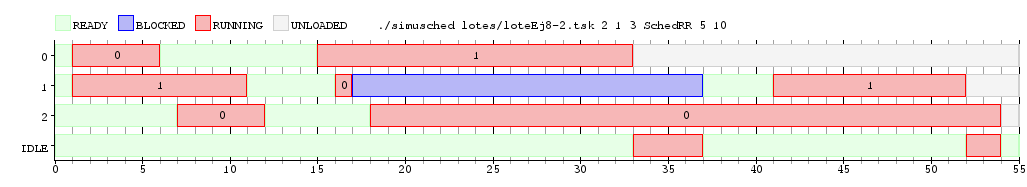
\includegraphics[width=1\textwidth]{img/imgEj8-1}
  \caption{}
  \label{fig:ej8-1}
\end{figure}



\begin{figure}[H]
  \centering
  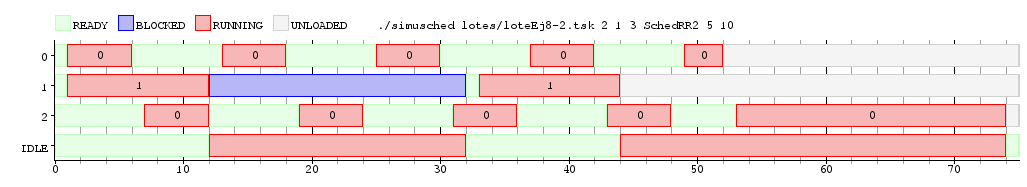
\includegraphics[width=1\textwidth]{img/imgEj8-2}
  \caption{}
  \label{fig:ej8-2}
\end{figure}



\begin{figure}[H]
  \centering
  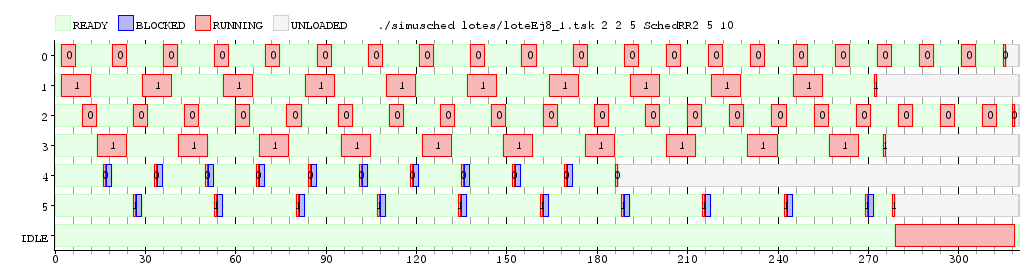
\includegraphics[width=1\textwidth]{img/imgEj8-3}
  \caption{}
  \label{fig:ej8-3}
\end{figure}



\begin{figure}[H]
  \centering
  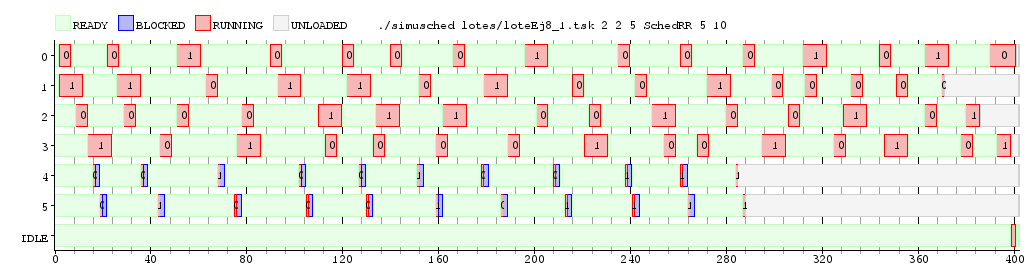
\includegraphics[width=1\textwidth]{img/imgEj8-4}
  \caption{}
  \label{fig:ej8-4}
\end{figure}












\newpage

\end{document}
